% Options for packages loaded elsewhere
\PassOptionsToPackage{unicode}{hyperref}
\PassOptionsToPackage{hyphens}{url}
\documentclass[
  ignorenonframetext,
]{beamer}
\newif\ifbibliography
\usepackage{pgfpages}
\setbeamertemplate{caption}[numbered]
\setbeamertemplate{caption label separator}{: }
\setbeamercolor{caption name}{fg=normal text.fg}
\beamertemplatenavigationsymbolsempty
% remove section numbering
\setbeamertemplate{part page}{
  \centering
  \begin{beamercolorbox}[sep=16pt,center]{part title}
    \usebeamerfont{part title}\insertpart\par
  \end{beamercolorbox}
}
\setbeamertemplate{section page}{
  \centering
  \begin{beamercolorbox}[sep=12pt,center]{section title}
    \usebeamerfont{section title}\insertsection\par
  \end{beamercolorbox}
}
\setbeamertemplate{subsection page}{
  \centering
  \begin{beamercolorbox}[sep=8pt,center]{subsection title}
    \usebeamerfont{subsection title}\insertsubsection\par
  \end{beamercolorbox}
}
% Prevent slide breaks in the middle of a paragraph
\widowpenalties 1 10000
\raggedbottom
\AtBeginPart{
  \frame{\partpage}
}
\AtBeginSection{
  \ifbibliography
  \else
    \frame{\sectionpage}
  \fi
}
\AtBeginSubsection{
  \frame{\subsectionpage}
}
\usepackage{iftex}
\ifPDFTeX
  \usepackage[T1]{fontenc}
  \usepackage[utf8]{inputenc}
  \usepackage{textcomp} % provide euro and other symbols
\else % if luatex or xetex
  \usepackage{unicode-math} % this also loads fontspec
  \defaultfontfeatures{Scale=MatchLowercase}
  \defaultfontfeatures[\rmfamily]{Ligatures=TeX,Scale=1}
\fi
\usepackage{lmodern}
\ifPDFTeX\else
  % xetex/luatex font selection
\fi
% Use upquote if available, for straight quotes in verbatim environments
\IfFileExists{upquote.sty}{\usepackage{upquote}}{}
\IfFileExists{microtype.sty}{% use microtype if available
  \usepackage[]{microtype}
  \UseMicrotypeSet[protrusion]{basicmath} % disable protrusion for tt fonts
}{}
\makeatletter
\@ifundefined{KOMAClassName}{% if non-KOMA class
  \IfFileExists{parskip.sty}{%
    \usepackage{parskip}
  }{% else
    \setlength{\parindent}{0pt}
    \setlength{\parskip}{6pt plus 2pt minus 1pt}}
}{% if KOMA class
  \KOMAoptions{parskip=half}}
\makeatother
\usepackage{graphicx}
\makeatletter
\newsavebox\pandoc@box
\newcommand*\pandocbounded[1]{% scales image to fit in text height/width
  \sbox\pandoc@box{#1}%
  \Gscale@div\@tempa{\textheight}{\dimexpr\ht\pandoc@box+\dp\pandoc@box\relax}%
  \Gscale@div\@tempb{\linewidth}{\wd\pandoc@box}%
  \ifdim\@tempb\p@<\@tempa\p@\let\@tempa\@tempb\fi% select the smaller of both
  \ifdim\@tempa\p@<\p@\scalebox{\@tempa}{\usebox\pandoc@box}%
  \else\usebox{\pandoc@box}%
  \fi%
}
% Set default figure placement to htbp
\def\fps@figure{htbp}
\makeatother
\setlength{\emergencystretch}{3em} % prevent overfull lines
\providecommand{\tightlist}{%
  \setlength{\itemsep}{0pt}\setlength{\parskip}{0pt}}
% Slide layout defaults for warning-clean scientific decks.
\usepackage{etoolbox}
\IfFileExists{xurl.sty}{\usepackage{xurl}}{}
\IfFileExists{seqsplit.sty}{\usepackage{seqsplit}}{\newcommand{\seqsplit}[1]{#1}}
\protected\def\breakseq#1{\seqsplit{#1}}
\protected\def\breaktt#1{\begingroup\ttfamily\seqsplit{#1}\endgroup}
\setlength{\emergencystretch}{6em}
\tolerance=5000
\hbadness=10000
\hfuzz=1pt
\setlength{\tabcolsep}{2pt}
\AtBeginEnvironment{longtable}{\tiny\renewcommand{\arraystretch}{0.86}\setlength{\tabcolsep}{1pt}}
\AtBeginEnvironment{tabular}{\tiny\renewcommand{\arraystretch}{0.86}\setlength{\tabcolsep}{1pt}}

% Natbib and cross-reference fallbacks — slides don't load natbib
% or cleveref, but combined-PDF manuscript prose may emit these
% commands. The fallback renders citations as a bracketed key list
% and cross-references as detokenized labels so slides don't fail on
% undefined control sequences or raw underscores. \providecommand is
% a no-op if packages load later.
\providecommand{\citep}[1]{[#1]}
\providecommand{\citet}[1]{#1}
\providecommand{\citealp}[1]{#1}
\providecommand{\citeauthor}[1]{#1}
\providecommand{\citeyear}[1]{#1}
\providecommand{\cref}[1]{\texttt{\detokenize{#1}}}
\providecommand{\Cref}[1]{\texttt{\detokenize{#1}}}

\newtheorem{proposition}{Proposition}
\newtheorem{hypothesis}{Hypothesis}
\usepackage{bookmark}
\IfFileExists{xurl.sty}{\usepackage{xurl}}{} % add URL line breaks if available
\urlstyle{same}
% fallback for those not using the hyperref driver hyperxmp:
\makeatletter
\@ifundefined{xmpquote}{\newcommand{\xmpquote}[1]{#1}}{}
\makeatother
\hypersetup{
  hidelinks,
  pdfcreator={LaTeX via pandoc}}

\author{\texorpdfstring{}{}}
\date{}

\begin{document}

\section{Accessible Shared Drawing: Capability Before
Claim}\label{sec:accessibility}

\begin{frame}[fragile,allowframebreaks]{Accessible Shared Drawing:
Capability Before Claim}
The original PPPiP emphasized low cost, but DigiPPPiP must treat
disability access as a first-order constraint rather than an
accommodation afterthought. Digital art therapy and telehealth
arts-therapy research show that online and digital modalities can expand
participation for people whose access needs make conventional studio or
clinic settings difficult, while also introducing pragmatic and ethical
constraints \breakseq{[@zubala2021digitalarttherapy; @reitere2024telehealth;
@potash2020pandemics]}. Online art-therapy work with learning-disabled
young adults also shows why the platform, group norms, and communication
channel are part of access rather than neutral delivery infrastructure
\breakseq{[@datlen2020whatsapp]}. Reframing digital art therapy for digitally
mediated practice adds the same structural warning: technology changes
the therapeutic and relational triangle rather than simply transporting
a studio session online \breakseq{[@haywood2022hexagonal]}. Accessibility here
is not merely compliance; it changes what kinds of relational drawing
become possible. Ability-based design and World Wide Web Consortium
(W3C) accessibility guidance support this shift from generic interface
polish toward capability-specific accommodation, including the Web
Content Accessibility Guidelines (WCAG) and the Cognitive and Learning
Disabilities Accessibility Task Force guidance (COGA)
\breakseq{[@wobbrock2011ability; @w3c2023wcag22; @w3c2021coga]}. Participatory
design work with children with special needs shows why access claims
should be made with the people affected rather than inferred from
designer intent \breakseq{[@frauenberger2011participatory]}. Social
accessibility research on assistive technology also shows that access is
shaped by self-presentation, confidence, stigma, and the social meaning
of visible supports \breakseq{[@shinohara2016socialaccess]}.

Inclusive DigiPPPiP should support multiple input channels: stylus,
touch, mouse, eye gaze, switch control, voice, assisted drawing, and
partner-mediated contribution. It should support multiple feedback
channels: visual stroke changes, haptic cues, audio descriptions,
high-contrast modes, and replayable action histories.
Accessible-visualization research adds an implementation lesson for the
figures and the drawing interface: nonvisual access needs navigable
structure, multimodal input, semantic rendering, and customizable text
tokens rather than a static image label \breakseq{[@elavsky2024datanavigator;
@jones2024customization]}. Plain-language controls matter because the
original practice made artistic skill non-essential; the digital
successor should also make technical skill non-essential. The audit
protocol in \breakseq{[@sec:methods\_protocol]} keeps these claims bounded to
visible capabilities instead of claiming universal access.

In protocol terms, access should be documented before the session,
during the session, and after the session. Before drawing, participants
should be able to state preferred input methods, perceptual feedback,
pacing, break needs, plain-language prompts, and partner-assistance
boundaries without having to disclose a diagnosis. During drawing, the
interface should log which accommodations were available and which were
actually used, because a capability advertised but unavailable in the
session cannot support an access claim. After drawing, participants
should be able to review whether the accommodation preserved agency,
privacy, and relational comfort rather than merely allowing task
completion.

The access requirement is deeper than device compatibility. A
participant must be able to initiate a mark, perceive the partner's
contribution, understand the session state, control persistence, and
remain socially comfortable with the accommodation used. Image-heavy
social systems can exclude blind users when visual content is not made
semantically available \breakseq{[@morris2016pictures]}. At the same time,
accessibility is often co-produced among disabled and nondisabled
companions in concrete settings rather than solved by a single feature
\breakseq{[@branham2015collaborativeaccess]}. If any of those conditions fails,
the system may be technically accessible while relationally
exclusionary. This is why the manuscript treats social accessibility as
part of the design problem rather than a secondary usability issue.

\breakseq{[@fig:accessibility\_features\_overview]} translates those domains
into implementation-facing commitments. The central point is not that
the current framework is accessible for every user; it is that each
access feature should be traceable to a partner need, a logged
capability, and a participatory validation plan.

\begin{figure}
\centering
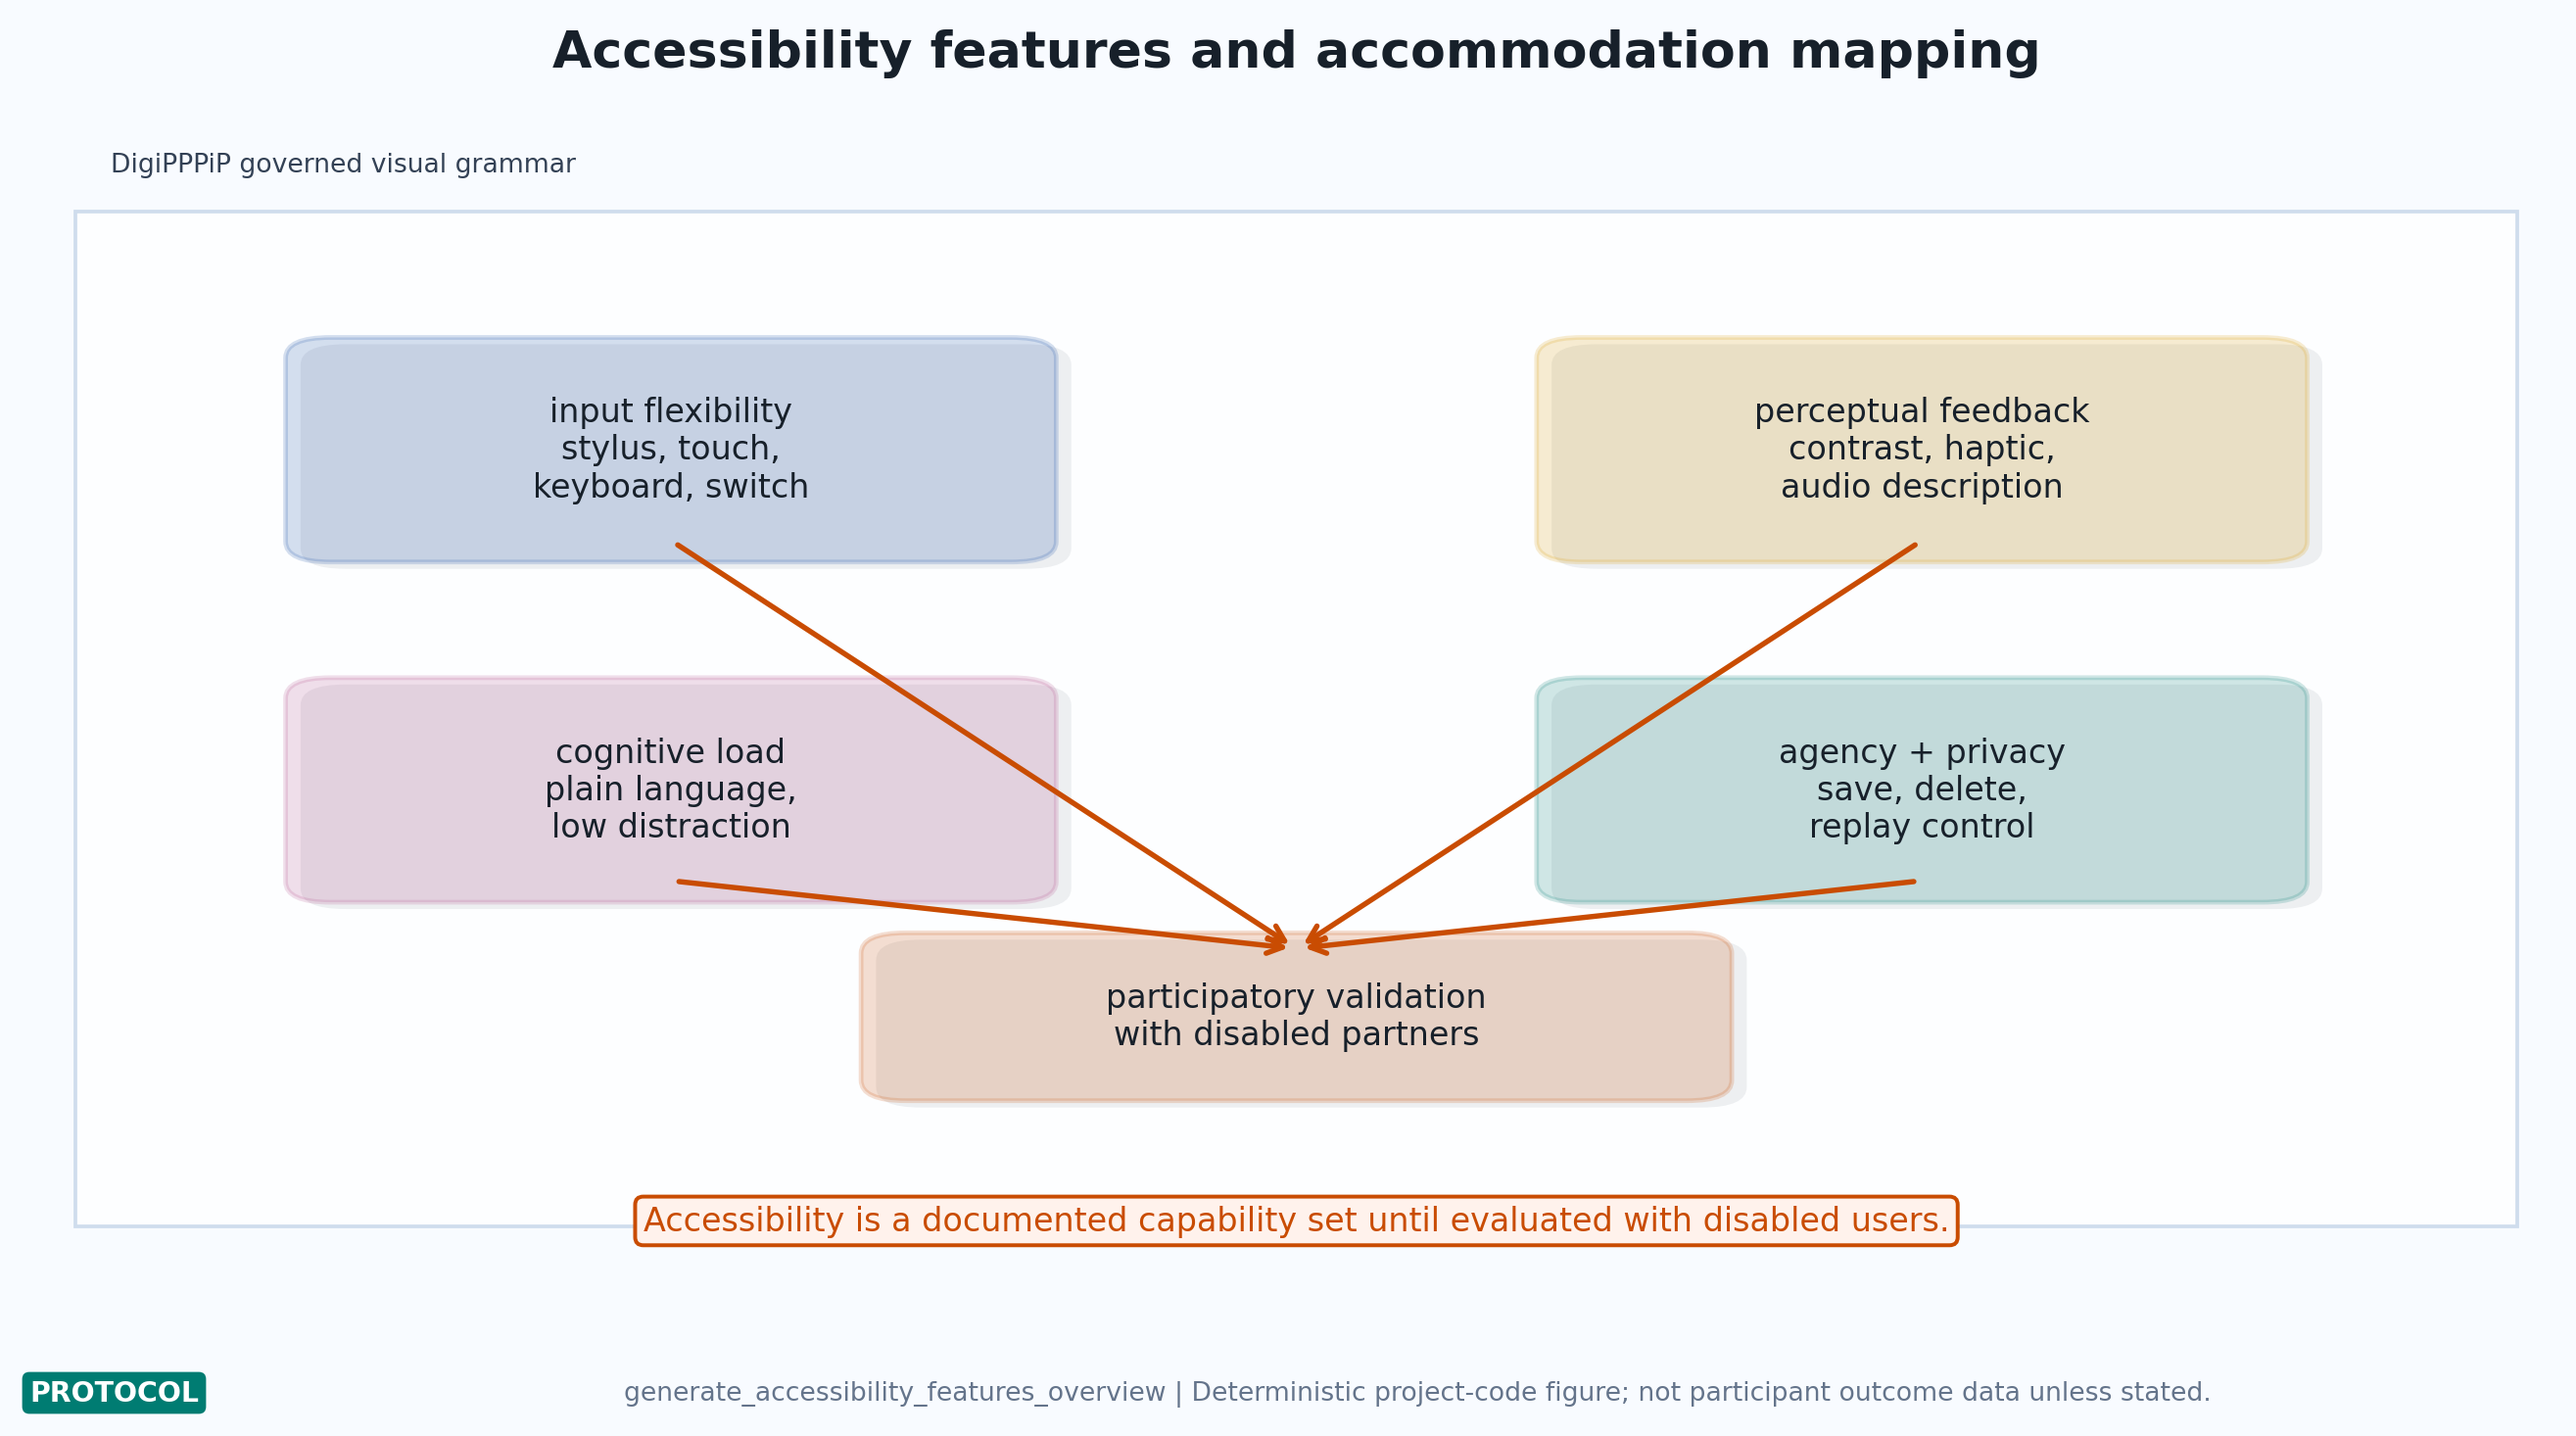
\includegraphics[width=0.9\linewidth,height=0.46\textheight,keepaspectratio,alt={Accessibility feature map linking input flexibility, perceptual feedback, cognitive-load control, and privacy agency to participatory validation. The figure is generated by generate\_accessibility\_features\_overview(); read each box as an implementation commitment that must point toward the central validation requirement with disabled partners, with accessible visualization scholarship motivating structured descriptions and customizable reading order. It supports the accessibility section's distinction between capability documentation and access claims. The diagram is conceptual and does not certify compliance or universal usability.}]{../figures/accessibility_features_overview.png}
\caption{Accessibility feature map linking input flexibility, perceptual
feedback, cognitive-load control, and privacy agency to participatory
validation. The figure is generated by
\protect\breaktt{generate\_accessibility\_features\_overview()}; read
each box as an implementation commitment that must point toward the
central validation requirement with disabled partners, with accessible
visualization scholarship motivating structured descriptions and
customizable reading order. It supports the accessibility section's
distinction between capability documentation and access claims. The
diagram is conceptual and does not certify compliance or universal
usability.}\label{fig:accessibility_features_overview}
\end{figure}

Accessibility also includes relational safety. Partners need control
over saving, sharing, replaying, exporting, deleting, and annotating a
canvas. The persistent archive that makes asynchronous DigiPPPiP
powerful can become invasive if consent and privacy are weak. The
research agenda in \breakseq{[@sec:agenda]} therefore treats participatory
design with disabled partners as a core empirical priority rather than a
platform feature request.
\end{frame}

\end{document}
